\section{Top Level Section}
\blindmathtrue
\blindtext

Ø£¢¥
äáàñæø

See my cool truth table (\ref{tab:truthy})

\begin{table} [h!]
\centering
\begin{minipage}{5cm}
\caption[Table \thetable. Truth Table]{ \textbf{A Truth Table.} } 
\begin{tabular} {c c c | c}
p & q & r & S\\ \hline
1 & 1 & 1 & 1\\
1 & 1 & 0 & 1\\
1 & 0 & 1 & 1\\
1 & 0 & 0 & 1\\
0 & 1 & 1 & 1\\
0 & 1 & 0 & 1\\
0 & 0 & 1 & 1\\
0 & 0 & 0 & 1\\
\end{tabular}
\label{tab:truthy}
\end{minipage}
\end{table}

\blindtext

And see my cool Cubehelix Graph (\ref{fig:cubehelix}).

\begin{figure}[!ht]
	\centering
	\begin{minipage}{10cm}
	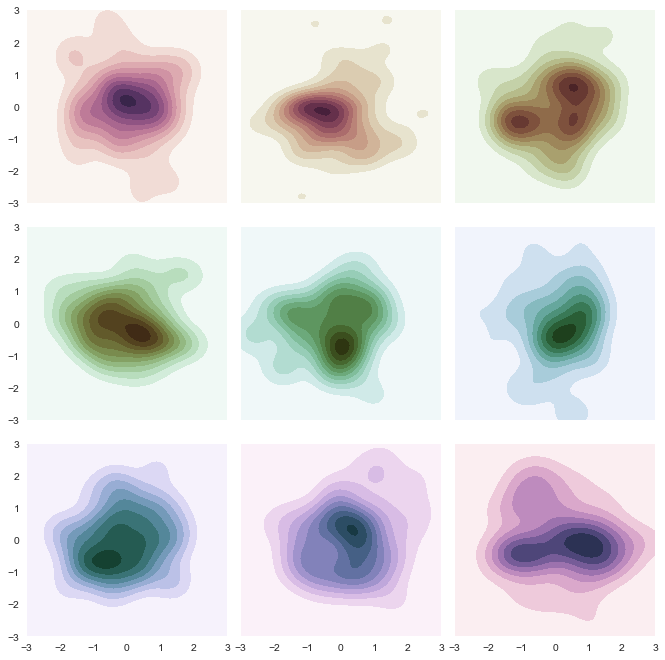
\includegraphics[width=\linewidth]{cubehelixpalette}
	\caption[Figure \thefigure. Cubehelix Graph]{ \textbf{Cubehelix Graph.} \textit{This is some caption text.}}
	\label{fig:cubehelix}
	\end{minipage}
\end{figure}

This is a citation\cite[chapter, p.~15]{greenwade93}.
And another citation\cite{goossens93}.

\begin{figure}[!ht]
	\centering
	\begin{minipage}{10cm}
	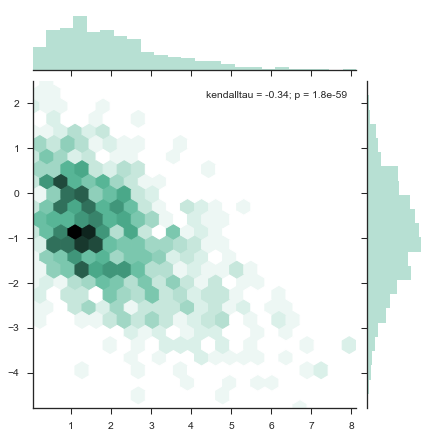
\includegraphics[width=\linewidth]{hexbinmarginals}
	\caption[Figure \thefigure. Hexbin Marginal Graph]{ \textbf{Hexbin Graph.} }
	\label{fig:hexbin}
	\end{minipage}
\end{figure}

Here is a crazy equation in \LaTeX
\begin{equation} \label{eq:crazy}
	\frac{\sin(2x + \pi)}{\cos(\int_0^\infty{\lambda_1 + \lambda_2})}
\end{equation}

See crazy equation (\ref{eq:crazy}).
